\chapter{Derivatives}

In calculus, the derivative of a function represents the rate at which the 
function is changing at a particular point. It is a fundamental concept that 
has vast applications in various fields, including physics.\index{derivative}

\section{Definition}

The derivative of a function $f(x)$ at a point $x$ is defined as the limit:

\begin{equation}
f'(x) = \lim_{{h \to 0}} \frac{f(x+h) - f(x)}{h}
\end{equation}

provided this limit exists. In other words, the derivative of $f$ at $x$ is the 
limit of the rate of change of $f$ at $x$ as the change in $x$ approaches zero. 
The derivative of a function is equal to the slope  of the function. 

Where does the definition of a derivative come from? Consider the function 
$f(x) = x^2$. Suppose we want to write an equation for a line that is tangent 
to the curve at $x = 2$ (see figure \ref{fig:tangent}). We already have a 
point that the line passes through: $(2, 4)$. To write an equation for the 
tangent line, we would need to know its slope, $m$. 

\begin{figure}[htbp]
    \centering
    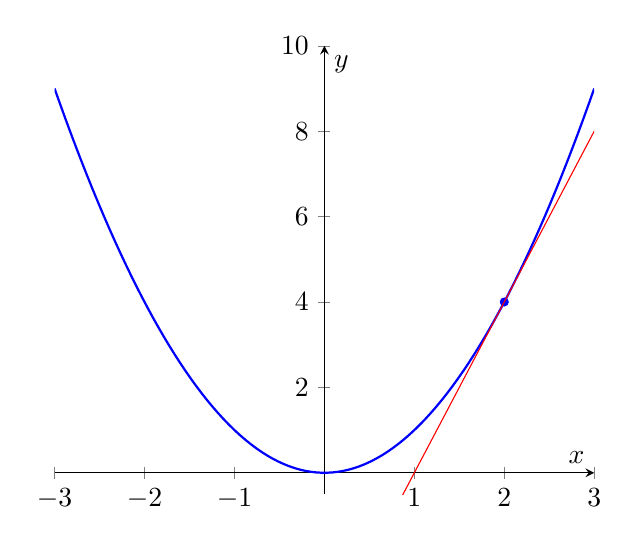
\begin{tikzpicture}
        \begin{axis}[axis lines = center, xmin = -3, xmax = 3, ymin = -0.5, 
        ymax = 10, xlabel = $x$, ylabel = $y$]
            \addplot[blue, thick, samples = 100, domain = -3:3]{x^2};
            \draw[blue, fill = blue] (2, 4) circle (0.5mm);
            \addplot[red, thin]{4*(x - 2) + 4};
        \end{axis}
    \end{tikzpicture}
    \caption{The red line is tangent to $f(x) = x^2$ at the point $(2, 4)$}
    \label{fig:tangent}
\end{figure}

We can estimate the slope by choosing another point, $Q$, near our known 
point, $P = (2, 4)$, and drawing a secant line through $P$ and $Q$ (see figure 
\ref{fig:secant}). Using the slope formula, $m = \left( y_2 - y_1 \right) / 
\left( x_2 - x_1 \right)$, we can find the slope of the secant line. 

\begin{figure}[htbp]
    \centering
    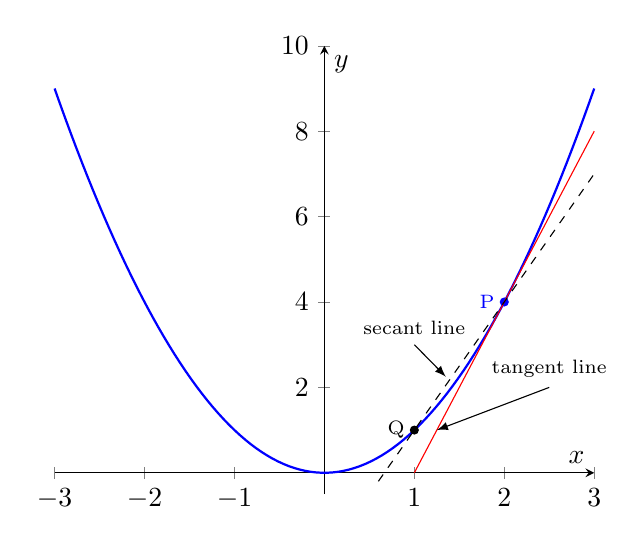
\begin{tikzpicture}
        \begin{axis}[axis lines = center, xmin = -3, xmax = 3, ymin = -0.5, 
        ymax = 10, xlabel = $x$, ylabel = $y$, clip = false]
            \addplot[blue, thick, samples = 100, domain = -3:3]{x^2};
            \draw[blue, fill = blue] (2, 4) circle (0.5mm) node[left, font = 
            \scriptsize] {P};
            \addplot[red, thin, domain = 1:3]{4*(x - 2) + 4};
            \draw[black, fill = black] (1, 1) circle (0.5mm) node[left, font = 
            \scriptsize] {Q};
            \addplot[black, thin, dashed, domain = 0.6:3]{3*(x - 2) + 4};
            \draw[latex-, black] (1.35, 2.25) -- (1, 3) node[above, font = 
            \scriptsize] {secant line};
            \draw[latex-, black] (1.25, 1) -- (2.5, 2) node[above, font = 
            \scriptsize] {tangent line};
        \end{axis}
    \end{tikzpicture}
    \caption{The slope of the secant line is approximately the slope of the 
    tangent line}
    \label{fig:secant}
\end{figure}

As $Q$ moves closer to $P$, the slope of the secant line is a better and 
better approximation of the slope of the tangent line (see figure fixme figure showing zoomed in about $P$ and several $Q$s moving closer to $P$ from either side of $P$). 

Much scientific data is not described as continuous functions, but rather as 
discreet data points. Consider the following data of a falling object:
\begin{center}
\begin{tabular}{|c|c|}
\hline
time (seconds) & height (m)\\\hline
0 & 50\\\hline
0.5 & 48.775\\\hline
1 & 45.1\\\hline
1.5 & 38.975\\\hline
2 & 30.4\\\hline
2.5 & 19.375\\\hline
3 & 5.9 \\\hline
\end{tabular}
\end{center}

A graph of the data is shown in figure \ref{fig:falling}.

\begin{figure}[htbp]
    \centering
    \begin{tikzpicture}
        \begin{axis}[axis lines = center, xmin = -0.5, xmax = 3.5, ymin = 
        -0.5, ymax = 52, xlabel = time(sec), ylabel = height(m)]
            \draw[blue, fill = blue] (0, 50) circle (0.7mm);
            \draw[blue, fill = blue] (0.5, 48.775) circle (0.7mm);
            \draw[blue, fill = blue] (1, 45.1) circle (0.7mm);
            \draw[blue, fill = blue] (1.5, 38.975) circle (0.7mm);
            \draw[blue, fill = blue] (2, 30.4) circle (0.7mm);
            \draw[blue, fill = blue] (2.5, 19.375) circle (0.7mm);
            \draw[blue, fill = blue] (3, 5.9) circle (0.7mm);
        \end{axis}
    \end{tikzpicture}
    \caption{The height of a falling object over time}
    \label{fig:falling}
\end{figure}

\begin{Exercise}[label=slope1]
	[This question was originally presented as a free-response, calculator-allowed 
	question on the 2012 AP Calculus BC Exam.] The temperature of water in a tub 
	at time $t$ is modeled by a function, $W$, where $W(t)$ is measured in degrees 
	Fahrenheit, and $t$ is measured in minutes. Values of $W(t)$ at selected times 
	for the first 20 minutes are given in the table. Use the data in the table to 
	estimate $W'(12)$. Show the computations that lead to your answer. Using 
	correct units, interpret the meaning of your answer in the context of the 
	problem. \\
	\begin{tabular}{c|c}\hline
	$t$ (minutes) & $W(t)$ (degrees Fahrenheit)\\
	\hline
	0 & 55.0\\
	\hline
	4 & 57.1\\
	\hline
	9 & 61.8\\
	\hline
	15 & 67.9\\
	\hline
	20 & 71.0\\
	\hline
	\end{tabular}	 
\end{Exercise}

\begin{Answer}[ref=slope1]
	To estimate the slope at $t = 12$, we can use the data at $t = 9$ and $t = 
	15$. The slope of the line connecting those points is approximate of the 
	slope at $t = 12$. $$\frac{y_2 - y_1}{x_2 - x_1} = \frac{67.9 - 61.8}{15 - 9} 
	= \frac{6.1}{6} = 1.017$$ The units for the numerator are degrees Fahrenheit 
	and the units for the denominator are minutes. Therefore, the estimated slope has units 
	of degrees Fahrenheit per minute. This represents the change in temperature 
	of the water in the tub. When $t = 12$, the water in the tub is increasing in 
	temperature at about 1 degree Fahrenheit per minute. 
\end{Answer}

\section{Applications in Mathematics}
\subsection{l'Hospital's Rule}
Consider the function $h(x) = \frac{\ln{x}}{x-1}$. Suppose we are interested 
in the behavior of $h(x)$ around $x=1$. If we apply the Quotient Rule, we get 
an indeterminate result: $$\lim_{x \to 1}\frac{\ln{x}}{x-1} = \frac{0}{0}$$ 

Looking at the graph of $h(x)$ (see figure \ref{fig:lhospital}), we can guess 
that $\lim_{x \to 1} \frac{\ln{x}}{x-1} = 1$. 

\begin{figure}[htbp]
\centering
\begin{tikzpicture}
\begin{axis}
    [clip=true,
    xmin=0, xmax=4,
    ymin=0, ymax=4,
    axis lines=left
    ]
    \addplot[blue, domain=0.01:4, samples=100]{ln(x)/(x-1)};
    \addplot[samples=50, black, dashed] coordinates{(1, 0)(1,1)};
    \addplot[samples=50, black, dashed] coordinates{(0, 1)(1,1)};
    \addplot[mark=*, fill=white, draw=blue] coordinates{(1, 1)};
\end{axis}
\end{tikzpicture}
\caption{$h(x) = \frac{\ln{x}}{x - 1}$}
\label{fig:lhospital}
\end{figure}

Let's examine the numerator and denominator separately. We will define $f(x) = 
\ln{x}$ and $g(x) = x - 1$ (see figure \ref{fig:zoom1}). 

\begin{figure}[htbp]
\centering
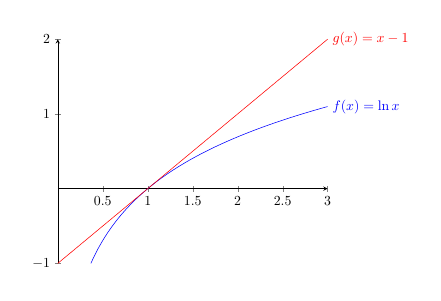
\begin{tikzpicture}[scale = 0.5]
    \begin{axis}
    [clip=false,
    xmin=0, xmax=3,
    ymin=-1, ymax=2,
    axis lines = center]
    \addplot[blue, samples=100, domain=1/e:3]{ln(x)}
    node[right, pos=1]{$f(x) = \ln{x}$};
    \addplot[red, samples=100, domain=0:3]{x-1}
    node[right, pos=1]{$g(x) = x - 1$};
    \end{axis}
\end{tikzpicture}
\caption{Examining each part of $\frac{\ln{x}}{x-1}$ separately}
\label{fig:zoom1}
\end{figure}

If we zoom in very close around $x=1$, the graphs begin to look linear (see 
figure \ref{fig:zoom2}):

\begin{figure}[htbp]
\centering
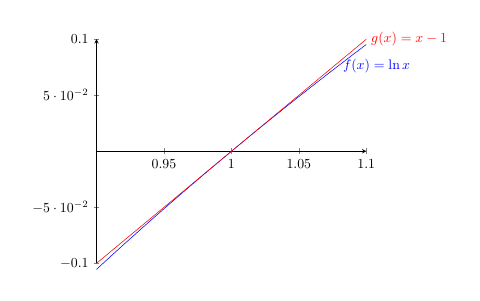
\begin{tikzpicture}[scale = 0.5]
    \begin{axis}
    [clip=false,
    xmin=0.9, xmax=1.1,
    ymin=-0.1, ymax=0.1,
    axis lines = center]
    \addplot[blue, samples=100, domain=0.9:1.1]{ln(x)}
    node[right, pos=0.9]{$f(x) = \ln{x}$};
    \addplot[red, samples=100, domain=0.9:1.1]{x-1}
    node[right, pos=1]{$g(x) = x - 1$};
    \end{axis}
\end{tikzpicture}
\caption{As we zoom in, the graph of $\ln{x}$ appears linear}
\label{fig:zoom2}
\end{figure}

We can approximate these graphs as linear functions with slopes $m_1$ and 
$m_2$, so that the blue curve is approximated as $y=m_1(x-1)$ and the red 
curve is approximated as $y=m_2(x-1)$. The ratio of the functions would then 
be 
$$\frac{m_1(x-1)}{m_2(x-1)}=\frac{m_1}{m_2}$$ 

which is the same as the ratio of the derivatives of our linear approximations. 
This suggests L'Hospital's rule, which is that the limit of a ratio is the same as the 
limit of the ratio of the derivatives for certain indeterminate forms: 
$$\lim_{x\to a}\frac{f(x)}{g(x)}=\lim_{x\to a}\frac{f'(x)}{g'(x)}$$.

Let's apply L'Hospital's rule to our limit of $h(x)$:
$$\lim_{x\to 1} \frac{\ln{x}}{x - 1} = \lim_{x \to 1} \frac{\frac{d}{dx} 
\ln{x}}{\frac{d}{dx} (x - 1)} = \lim_{x \to 1} \frac{\frac{1}{x}}{1}=1$$

Notice our result with L'Hospital's rule matches our guess based on the graph 
of $h(x) = \frac{\ln{x}}{x-1}$. 

L'Hospital's rule also applies to the indeterminate result $\frac{\pm \infty}
{\pm \infty}$. For a limit of the form $\lim_{x\to a}\frac{f(x)}{g(x)}$, 
L'Hospital's rule applies if:
\begin{enumerate}
    \item the original limit is of the indeterminate form $\frac{0}{0}$ or 
    $\frac{\pm \infty}{\pm \infty}$
    \item $f$ and $g$ are differentiable on an interval containing $a$ (but 
    possibly not differentiable at $a$)
    \item $g'(x) \neq 0$ on said interval
\end{enumerate}

\textbf{Example}: Determine $\lim_{x \to \infty} \frac{e^x}{x^2}$.

\textbf{Solution}: We begin by evaluating the limit:
$$\lim_{x \to \infty} \frac{e^x}{x^2} = \frac{e^{\infty}}{\infty^2} = 
\frac{\infty}{\infty}$$

This is an indeterminate form that we can apply L'Hospital's rule to:
$$= \lim_{x \to \infty} \frac{\frac{d}{dx}e^x}{\frac{d}{dx}x^2} = \lim_{x \to 
\infty} \frac{e^x}{2x}$$

Evaluating this limit, we get another indeterminate form:
$$=\frac{e^{\infty}}{2 \cdot \infty} = \frac{\infty}{\infty}$$

Don't panic! We can apply L'Hospital's rule again (in fact, we can apply 
L'Hospital's rule as many times as needed to evaluate a limit, as long as we 
keep getting $\frac{0}{0}$ or $\frac{\pm \infty}{\pm \infty}$):
$$= \lim_{x \to \infty} \frac{\frac{d}{dx}e^x}{\frac{d}{dx}2x} = \lim_{x \to 
\infty} \frac{e^x}{2} = \frac{\infty}{2} = \infty$$

and therefore, $\lim_{x \to \infty} \frac{e^x}{x^2} = \infty$.

\begin{Exercise}[label=LH1]
What is $\lim_{x \to 0} \frac{\tan{x} - x}{x^3}$?
\end{Exercise}

\begin{Answer}[ref=LH1]
First, let's confirm that L'Hospital's rule applies here:
$$\lim_{x \to 0} \frac{\tan{x} - x}{x^3} = \frac{0 - 0}{0} = \frac{0}{0}$$

Therefore, we can apply L'Hospital's rule:
$$\lim_{x \to 0} \frac{\tan{x} - x}{x^3} = \lim_{x \to 0} \frac{\frac{d}{dx}(\tan{x} - x)}{\frac{d}{dx}x^3}$$
$$= \lim_{x \to 0} \frac{\sec^2{x} - 1}{3x^2} = \frac{1 - 1}{0} = \frac{0}{0}$$

which is an indeterminate form. We apply L'Hospital's rule again:
$$\lim_{x \to 0} \frac{\tan{x} - x}{x^3} = \lim_{x \to 0} \frac{\frac{d}{dx}(sec^2{x} - 1)}{\frac{d}{dx}3x^2}$$
$$= \lim_{x \to 0} \frac{2\tan{x}\sec^2{x}}{6x} = \frac{2(0)(1^2)}{6 \cdot 0} = \frac{0}{0}$$

which is also an indeterminate form. We apply L'Hospital's rule again:
$$\lim_{x \to 0} \frac{\tan{x} - x}{x^3} = \lim_{x \to 0} \frac{\frac{d}{dx}(2\tan{x}\sec^2{x})}{\frac{d}{dx}6x}$$
$$= \lim_{x \to 0} \frac{2\sec^2{x}[2\tan^2{x} + \sec^2{x}]}{6} = \frac{2 \cdot 1 \cdot [2 \cdot 0 + 1]}{6}$$
$$= \frac{2}{6} = \frac{1}{3}$$
\end{Answer}

%fixme other indeterminite forms

\begin{Exercise}[label = LH2]
Evaluate each of the following limits, using L'Hospital's rule where needed.
\begin{enumerate}
\item $\lim_{x \to 3} \frac{x-3}{x^2-9}$
\item $\lim_{x \to 1/2} \frac{6x^2 + 5x - 4}{4x^2 + 16x - 9}$
\item $\lim_{x \to 0^+} \frac{\ln{x}}{\sqrt{x}}$
\item $\lim_{x \to \pi} \frac{1 + \cos{x}}{1 - \cos{x}}$
\item $\lim_{x \to 1} \frac{x\sin{x - 1}}{2x^2 - x - 1}$
\end{enumerate}
\end{Exercise}

\begin{Answer}[ref=LH2]
\begin{enumerate}
\item $\lim_{x \to 3} \frac{x-3}{x^2-9} = \frac{0}{0}$, so we apply L'Hospital's rule. $\lim_{x \to 3} \frac{x-3}{x^2-9} = \lim_{x \to 3} \frac{1}{2x} = \frac{1}{6}$
\item $\lim_{x \to 1/2} \frac{6x^2 + 5x - 4}{4x^2 + 16x - 9} = \frac{0}{0}$, so we apply L'Hospital's rule. $\lim_{x \to 1/2} \frac{6x^2 + 5x - 4}{4x^2 + 16x - 9} = \lim_{x \to 1/2} \frac{12x + 5}{8x + 16} = \frac{11}{20}$
\item $\lim_{x \to 0^+} \frac{\ln{x}}{\sqrt{x}} = \frac{-\infty}{0} = -\infty$. This limit does not require L'Hospital's rule because it is evaluable
\item $\lim_{x \to 1} \frac{x\sin{x - 1}}{2x^2 - x - 1} = \frac{1 \cdot \sin{1 - 1}}{2(1)^2 - 1 - 1} = \frac{0}{0}$, so we apply L'Hospital's rule: $\lim_{x \to 1} \frac{x\sin{x - 1}}{2x^2 - x - 1} = \lim_{x \to 1} \frac{\frac{d}{dx}(x\sin{x-1}}{\frac{d}{dx}(2x^2 - x - 1} = \lim_{x \to 1} \frac{x \cdot \cos{x - 1} + \sin{x - 1}}{4x - 1} = \frac{1 \cdot \cos{0} + \sin{0}}{4 - 1} = \frac{1 \cdot 1 + 0}{-3} = \frac{-1}{3}$. 
\end{enumerate}
\end{Answer}

\subsection{Mean Value Theorem}

The Mean Value Theorem (MVT) states that on an interval $[a, b]$ where a 
continuous function $f$ is differentiable on an open interval $(a, b)$, there 
is at least one point where the tangent line to $f$ has the same slope as a 
line connecting the points $(a, f(a))$ and $(b, f(b))$. Consider the graph of 
$f(x) = x^2$ (see figure \ref{fig:MVT1}). The line connecting the points 
$(-1, 1)$ and $(2, 4)$ has a slope of $\frac{1}{2}$. MVT tells us there must 
be \textit{at least one} point, $c$, on the interval $x \in (-1, 2)$ where 
$f'(c) = \frac{1}{2}$. We can find this point by setting $f'(x)$ equal to 
$\frac{1}{2}$: 
$$2x = \frac{1}{2} \rightarrow x = \frac{1}{4}$$

Examining the figure \ref{fig:MVT1}, you can see that the tangent at 
$f(\frac{1}{4})$ (the black line) is parallel to the red line connecting 
$(-1, f(-1))$ and $(2, f(2))$. 

\begin{figure}[htbp]
\begin{tikzpicture}
    \begin{axis}
        [ymin=-2, xmin=-2, xmax=2, axis lines = left]
        \addplot[blue, samples=50]{x^2};
        \addplot[red, mark=*]coordinates {(-1, 1)};
        \addplot[red, mark=*] coordinates {(2, 4)};
        \addplot[domain=-2:2, red] coordinates{(-1, 1)(2, 4)};
        \addplot[black, mark=*] coordinates{(0.5, 0.25)};
        \addplot[black, domain=-2:2, samples=50
        ]{x-0.25};
    \end{axis}
\end{tikzpicture}
\caption{$f(x) = x^2$}
\label{fig:MVT1}
\end{figure}

Note that MVT doesn't tell us \textit{where} $f'(x)$ is parallel to the line 
connecting $(a, f(a))$ and $(b, f(b))$, just that some value $c$ exists that 
satisfies the condition. 

\textbf{Example}: Consider a hammer thrown upwards at 5 $\frac{m}{s^2}$ on 
Earth (where the acceleration due to gravity is approximately $-9.8 
\frac{m}{s^2}$). 

\textbf{Solution}: We can use the MVT to show that there must be some point in 
the hammer's path upwards where the velocity of the hammer is exactly equal to 
its average velocity as it flies through the air. 

The hammer's rise can be described with the function $y(t) = 5t-4.9t^2$. The 
hammer reaches its peak at approximately $t=0.51$. So, we are looking for some 
value, $c$, such that $$y'(c) = \frac{y(0.51) - y(0)}{0.51 - 0} = \frac{5(0.51) 
- 4.9(0.51^2)}{0.51} = \frac{1.2755}{0.51} = 2.5$$

Solving $y'(t) = 5-9.8t = 2.5$, we find that the $c$ that satisfies the MVT is 
approximately $0.255$. This result is illustrated in figure \ref{fig:hammer}:

\begin{figure}[htbp]
\centering
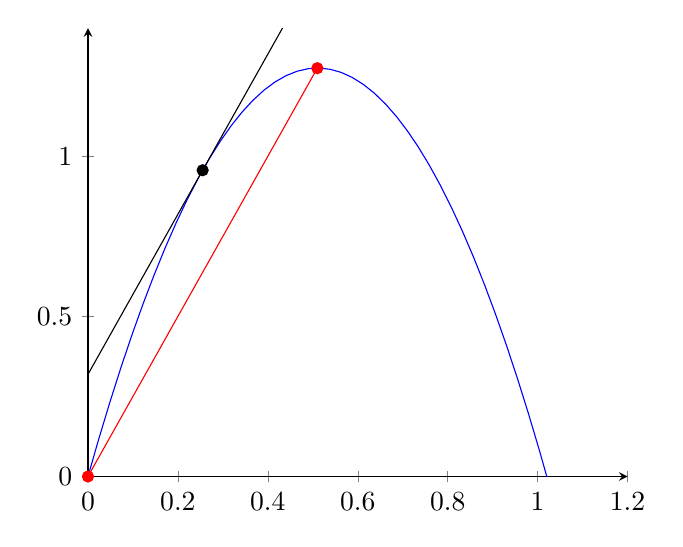
\begin{tikzpicture}
    \begin{axis}[ymin=0,ymax=1.4, xmin=0, xmax=1.2, axis lines=left]
    \addplot[blue, samples=50, domain=0:1.2]{5*x-4.9*x^2};
    \addplot[mark=*, red] coordinates{(0,0)};
    \addplot[mark=*, red] coordinates{(0.51, 1.275)};
    \addplot[red, samples=50]coordinates{(0,0) (0.51, 1.275)};
    \addplot[black, samples=50]{2.5*(x-0.255)+0.9564};
    \addplot[mark=*, black]coordinates{(0.255, 0.9564)};
    \end{axis}
\end{tikzpicture}
\caption{The height of a hammer tossed upwards at $5 \frac{m}{s}$}
\label{fig:hammer}
\end{figure}

\subsubsection{MVT Practice}
\begin{Exercise}
[label=MVT1]
At 3:30 PM, a car's speedometer reads $30 \frac{mi}{hr}$. At 3:40 PM, it reads 
$50\frac{mi}{hr}$. Show that at some time between 3:30 and 3:340 PM, the car's 
acceleration is exactly $120 \frac{mi}{hr^2}$. 
\end{Exercise}
\begin{Answer}
[ref=MVT1]
The speed of a car must be a continuous, differentiable function, since your car 
can't "jump" from one speed to another. Instead, it must smoothly accelerate from one 
speed to another. Therefore, the Mean Value Theorem applies. The average 
acceleration from 3:30 PM to 3:40 PM is given by:
$$\frac{\text{change in speed}}{\text{change in time}} = \frac{50 \frac{mi}{hr}
 - 30\frac{mi}{hr}}{3:40PM - 3:30PM}$$ 
Simplifying and converting minutes to hours, we see the average acceleration is:
$$\frac{20\frac{mi}{hr}}{\frac{1}{6}hr} = 120\frac{mi}{hr^2}$$

Therefore, by MVT, there must be some time between 3:30 and 3:40 PM where the 
car's acceleration is exactly $120 \frac{mi}{hr^2}$. 
\end{Answer}

\begin{Exercise}
[label=MVT2]
Find the number $c$ that satisfies the MVT on the given interval. 

(a) $f(x) = \sqrt{x}$, $[0, 4]$

(b)$f(x) = e^{-x}$, $[0,2]$

(c)$f(x) = \ln{x}$, $[1,4]$	
\end{Exercise}

\begin{Answer}
[ref=MVT2]
(a) For the domain given, $f(x)$ is defined and differentiable. Finding the 
slope of the secant line connecting the endpoints:
$$\frac{f(b)-f(a)}{b-a}=\frac{\sqrt{4}-\sqrt{0}}{4-0}=\frac{2}{4}=\frac{1}{2}$$

So, we are looking for some number $c$, such that $f'(c) = \frac{1}{2}$. Let's 
find $f'(x)$:
$$f'(x) = \frac{d}{dx}\sqrt{x}=\frac{1}{2\sqrt{x}}$$

Setting this equal to $\frac{1}{2}$ to find $c$:
$$f'(c) = \frac{1}{2\sqrt{c}}=\frac{1}{2}$$
$$\sqrt{c}=1$$
$$c=1$$

(b)For the domain given, $f(x)$ is defined and differentiable. Finding the 
slope of the secant line connecting the endpoints:
$$\frac{f(2) - f(0)}{2 - 0}=\frac{e^{-2} - e^{0}}{2}=\frac{1 - e^{2}}{2e^{2}} 
\approx -0.432$$

And find $f'(x)$:
$$f'(x) = -e^{-x}$$
According to MVT, there must be some $c$, such that $f'(c) \approx-0.432$:
$$-e^{-c} \approx -0.432$$
$$e^{-c}\approx 0.432$$
$$-c \approx \ln{0.432}$$
$$c \approx -\ln{0.432} \approx 0.839$$

(c) For the domain given, $f(x)$ is defined and differentiable. Finding the 
secant line connecting the endpoints:
$$\frac{f(b) - f(a)}{b - a}=\frac{\ln{4} - \ln{1}}{4 - 1} = \frac{\ln{4}}{3} 
\approx 0.462$$

And find $f'(x)$:
$$f'(x) = \frac{1}{x}$$

According to MVT, there must be some $c$ such that $f'(c) \approx 0.462$
$$f'(c) = \frac{1}{c} \approx 0.462$$
$$c \approx \frac{1}{0.462} = 2.164$$
\end{Answer}



\section{Applications in Physics}

In physics, derivatives play a vital role in describing how quantities change 
with respect to one another.

\subsection{Velocity and Acceleration}

In kinematics, the derivative of the position function with respect to time 
gives the velocity function, and further taking the derivative of the velocity 
function gives the acceleration function. For example, if $s(t)$ represents 
the position of an object at time $t$, then the velocity $v(t)$ and 
acceleration $a(t)$ are given by:

\begin{equation}
v(t) = \frac{ds}{dt} \quad \text{and} \quad a(t) = \frac{dv}{dt} = \frac{d^2s}{dt^2}
\end{equation}

\subsubsection{Practice}

A particle's motion is described by $s(t) = t^3-6t^2+6t$, where $t$ is measured 
in seconds and $s$ is measured in meters. Answer the following questions about 
the particle's motion:
\begin{Exercise}[label=velacc1]
Find the velocity at time $t$.
\end{Exercise}

\begin{Answer}[ref=velacc1]
Velocity is the derivative of position. Therefore, $v(t) = s'(t) = 3t^2-12t+6$.
\end{Answer}

\begin{Exercise}[label=velacc2]
What is the velocity after 2s? After 4s?
\end{Exercise}

\begin{Answer}[ref=velacc2]
$$v(2) = 3(2)^2-12(2)+6=-6 \frac{m}{s}$$
$$v(4) = 3(4)^2-12(4)+6=6\frac{m}{s}$$
\end{Answer}

\begin{Exercise}[label=velacc3]
When is the particle at rest?
\end{Exercise}

\begin{Answer}[ref=velacc3]
When the particle is at rest, $v(t) = 0$. 
$$3t^2-12t+6=0$$
$$3(t^2-4t+2)=0$$
$$t^2-4t+2=0$$
This is not easily factorable, so we will use the quadratic formula: $$t=\frac{-(-4)\pm\sqrt{(-4)^2-4(1)(2)}}{2(1)}$$
$$x=\frac{4\pm\sqrt{16-8}}{2}=2\pm\sqrt{2}\approx0.586, 3.414$$
Therefore, the particle is at rest at 0.586s and 3.414s.
\end{Answer}

\subsection{Force and Momentum}

In mechanics, the derivative of the momentum of an object with respect to time gives the net force acting on the object, as stated by Newton's second law of motion:

\begin{equation}
F = \frac{dp}{dt}
\end{equation}

where $F$ is the force, $p$ is the momentum, and $t$ is the time.
